\documentclass[%
        %draft,
        %submission,
        %compressed,
        final,
        %
        %technote,
        %internal,
        %submitted,
        %inpress,
        %reprint,
        %
        %titlepage,
        notitlepage,
        %anonymous,
        narroweqnarray,
        inline,
        %twoside,
        ]{ieee}

\usepackage{ieeefig}
\usepackage[utf8]{inputenc}
\usepackage{float}

\begin{document}

%----------------------------------------------------------------------
% Title Information, Abstract and Keywords
%----------------------------------------------------------------------
\title[Short Title]{Trabajo Práctico Nro 1: Wiretapping}

% format author this way for journal articles.
\author[SHORT NAMES]{%
      Christian Bonomi \small{LU:727/02},
    \and
      Claudio Gauna \small{LU:733/99},
    \and
      Marcelo Ferranti \small{LU:744/08},
    \and  
      Andrés Gutter \small{LU:007/08}
  }

% format author this way for conference proceeding

% specifiy the journal name
\journal{Teoría de las comunicaciones, 2016}

% Or, when the paper is a preprint, try this...
%\journal{IEEE Transactions on Something, 1997, TN\#9999.}

% Or, specify the conference place and date.

% make the title
\maketitle               

% do the abstract
\begin{abstract}

En este trabajo nos encargamos de implementar una serie de herramientas
para capturar los paquetes ARP de ciertas LANs, analizar las capturas
y tratar de inferir la topología de la red a partir de las mismas.
 
\end{abstract}

% do the keywords
\begin{keywords}
ARP, IP, MAC, Ethernet, Wi-Fi, Entropía, Fuente de información,
\end{keywords}

% start the main text ...
%----------------------------------------------------------------------
% SECTION I: Introduction
%----------------------------------------------------------------------

\section{Introducción}
\PARstart El objetivo principal de este trabajo práctico es averiguar de qué manera viaja un paquete que se envía 
desde un host hacia otro que está ubicado a una distancia geográfica considerable a través de Internet, 
que corresponde a la capa de Red dentro del modelo OSI.
Sabemos que cuando un host manda un paquete, éste último pasa a través de diferentes redes. Para lograr esto, 
vamos a crear una herramienta en Scapy que envía paquetes ICMP a una cierta dirección ip/web (de tres universidades ubicadas en el otro extremo del globo). 

Para dicho paquete, vamos a modificar incrementalmente el campo TTL (Time To Live). Éste es un campo que indica 
cuántos saltos entre red y red puede dar a lo sumo. Cuando no llega a destino debido a que no le alcanzó el TTL, 
retorna la cantidad de milisegundos que le tomó ir hasta donde pudo llegar y volver al host origen (RTT Round Trip Time)
y las coordenadas de geolocalización de la ip alcanzada.

\subsection{Instalación de librerias necesarias}

Para poder ejecutar la herramienta es necesario tener instaladas las siguientes librerias:

\subsubsection{GeoIP}
\begin{verbatim}
pip install pygeoip
\end{verbatim}

\subsubsection{Basemap}
\begin{verbatim}
sudo apt-get install python-mpltoolkits.basemap
\end{verbatim}
\section{Desarrollo}

\PARstart Para analizar la red se van a utilizar dos herramientas. Una que modela los paquetes Ethernet
capturados como una fuente de información binaria de memoria nula $S$, 
definiendo el conjunto de símbolos que emite como ${S_{BROADCAST}, S_{UNICAST}}$.
La segunda herramienta modela una fuente de información de memoria nula $S1$ 
que emite símbolos que son la IP destino de los paquetes $ARP$ de tipo $Who-has$ capturados. La herramienta que modela esta fuente no tiene en cuenta los paquetes ARP gratuitos, ya que estos no son necesarios por el standar de ARP (RFC 826), pero si pueden ser utilizados en otros casos, para detectar conflictos de ip, para que otras maquinas hagan un update de su tabla, o cuando se levanta una interfaz de red. Al sacar estos paquetes podemos focalizarnos en analizar los paquetes $ARP$ $Who-has$ que efectivamente estan preguntado por una ip desconocida.
Un símbolo de esta fuente será distinguido cuando la información provista
por el símbolo sea menor que la entropía de la fuente.

\subsection{Descripción y uso de la implementación} 
El código esta en dos carpetas $shared$ y $entregable$.\\

En la carpeta $shared$ estan los siguientes archivos:

\begin{itemize}
\item fuente.py. Tiene los metodos para crear las fuentes a partir de los paquetes. También tiene funciones para calcular la entropia, entropia maxima e informacion de los simbolos.
\item grafo.py. Tiene los metodos para crear y graficar el grafo de la red.
\item graficos.py. Tiene los metodos para graficar los histogramas de los simbolos de una fuente.
\item reader.py. Tiene los metodos para hacer sniff online y offline.
\end{itemize}

En la carpeta $entregable$ esta elarchivo $tp1.py$ que es el script principal que tiene todo el codigo para generar las fuentes $S$ y $S1$ con sus respectivos graficos y la imagen del grafo de la red.\\

La forma de uso es la siguiente:

\textit{sudo python tp1.py --online file.pcap}.\\
\textit{python tp1.py --offline file.pcap}.

\section{Red laboratorio}

Para este experimento se tomo una captura de 30 minutos de la red Wi-Fi de los labos de la facultad.

\begin{figure}[h]
  \centering
    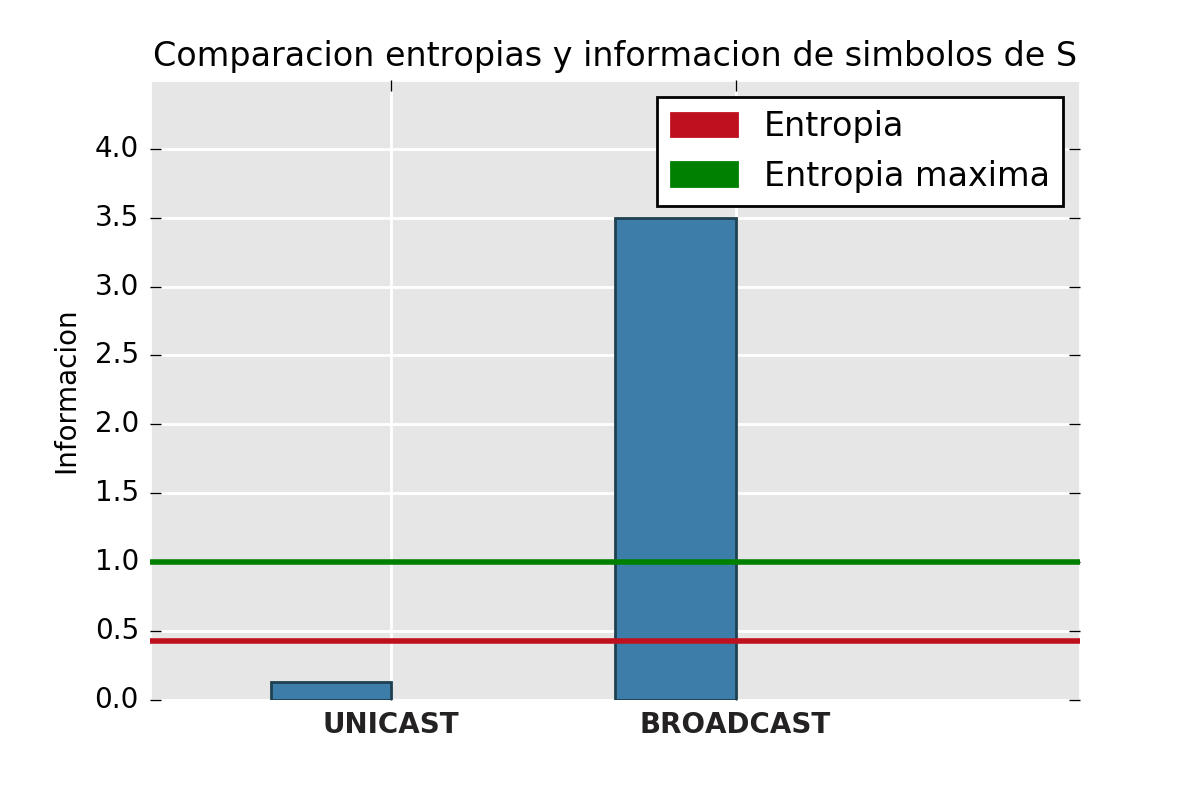
\includegraphics[width=0.45\textwidth]{grafico1-red-labos.png}
  \caption{Entropia de la fuente}
  \label{entropia-s}
\end{figure}

Como podemos ver en el gráfico comparativo la entropía no llega a ser máxima. De hecho puede verse en el símbolo $BROADCAST$ proporciona mucha mas información que el símbolo $UNICAST$. 

Por lo que hay un mayor flujo de paquetes Ethernet $UNICAST$ que $BROADCAST$, esto podría deberse a cambios en la topología de la red.

Dado que esta es una red Wi-fi, se esperaría que haya muchos dispositivos conectandose y desconectandose, con lo cual es muy factible que la topología de la red vaya variando a lo largo del tiempo.

Los cambios de topología redicen el tiempo de las entradas en la tabla CAM en el caso de Spanning Tree Protocol. En redes que hacen uso de Rapid Spanning Tree Protocol, las direcciones MAC se liberan de la tabla CAM de forma inmediata.


    \begin{table}[ht]\begin{center}
      \begin{tabular}{|c|c|}
      \hline
      \textbf{Nodo} & \textbf{Información} \\ \hline
      \texttt{UNICAST}& 0.133654 \\ \hline
      \texttt{BROADCAST}& 3.498507 \\ \hline
      \end{tabular}
      \caption{Información de los símbolos de S}
      \label{info-simbolos}
    \end{center}\end{table}


El overhead impuesto por la red influencia la entropía de esta fuente.
Por ejemplo, si hubiese mas mensajes $ARP$ $BROADCAST$ la información del símbolo $S_{BROADCAST}$ bajaría haciendo consecuentemente que la entropía de la fuente $S$ se vea modificada.

\begin{figure}[h]
  \centering
    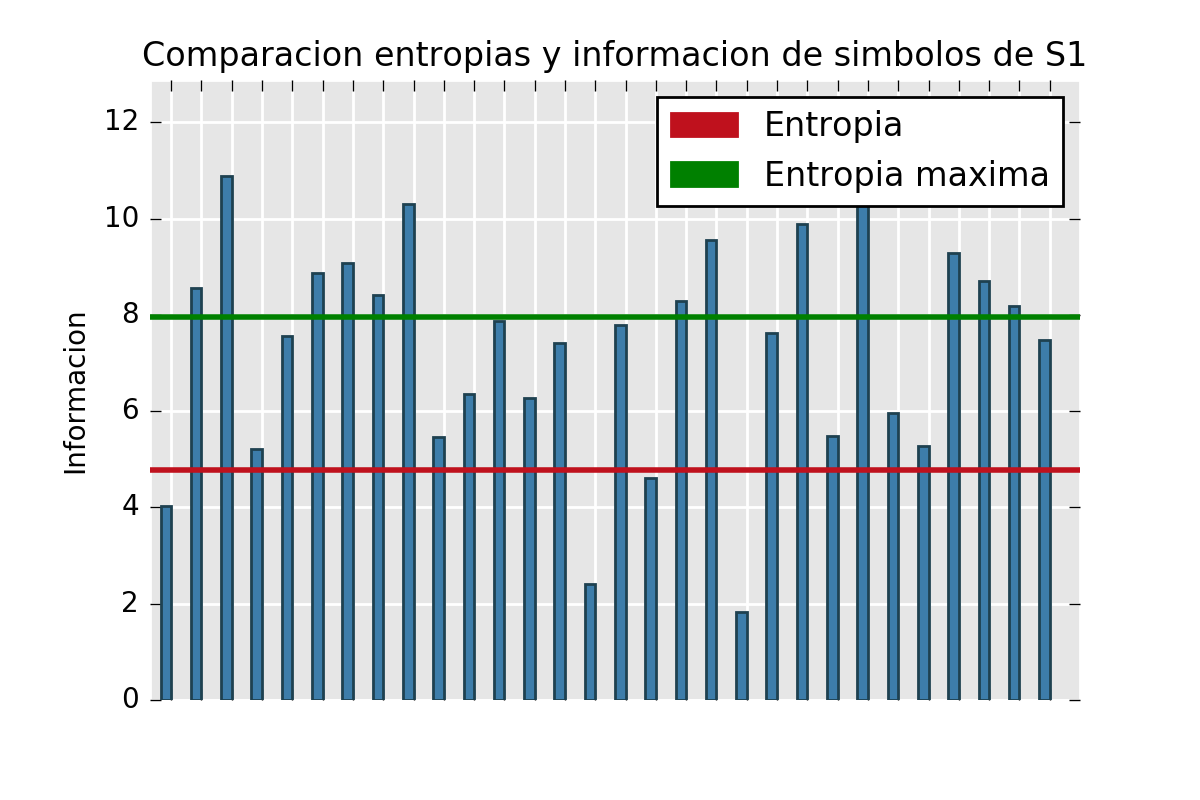
\includegraphics[width=0.45\textwidth]{grafico2-red-labos.png}
  \caption{Entropia de la fuente S1}
  \label{entropia-s1}
\end{figure}
En este gráfico agrupamos la información puesto que había demasiados símbolos.

En comparación con el resto de los mensajes el tráfico $ARP$ es bajo, sólo el 4\% de los mensajes son $ARP$. En base al criterio propuesto, se pueden distinguir 4 nodos, que en el grafico se corresponden con las cuatro barras que están por debajo de la entroppía de la fuente:   

    \begin{table}[ht]\begin{center}
      \begin{tabular}{|c|c|}
      \hline
      \textbf{Nodo} & \textbf{Informacion} \\ \hline
      \texttt{10.2.7.254}& 1.829564 \\ \hline
      \texttt{10.2.203.254}& 2.414527 \\ \hline
      \texttt{10.2.1.250}& 4.026302 \\ \hline
      \texttt{10.2.3.254}& 4.601927 \\ \hline
      \end{tabular}
      \caption{Nodos destacados}
      \label{Nodos-destacados}
    \end{center}\end{table}

Como en nuestra fuente estamos tomando las IPs destino de los paquetes $ARP$ $Who-has$. Esto indíca que estas IPs son muy frecuentes con lo cual se podría pensar en el escenario en que la mayoría de los nodos quiere conocer la MAC del Default Gateway por lo tanto envían tramas $Who-has$ con la dirección destino del mismo.

Por lo tanto bajo ese escenario estos cuatro nodos distinguidos podrían ser Default Gateway/s. 


\begin{figure}[h]
  \centering
    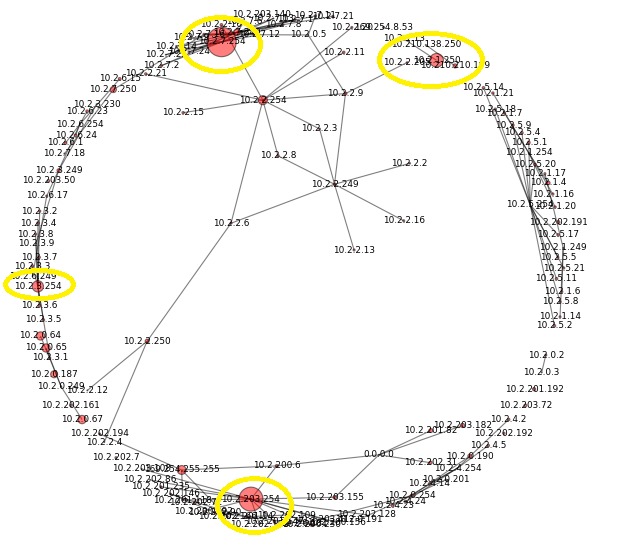
\includegraphics[width=0.45\textwidth]{grafo-red-labos-destacados.png}
  \caption{Grafo de la fuente S1}
  \label{grafo-s1}
\end{figure}

Los nodos remarcados son los posibles Default Gateway.
\section{Red oficina}

Para este experimento se tomo una captura de 30 minutos de la red Wi-Fi la oficina de taringa.
La oficina al momento de la captura contaba con unas 20 personas conectadas a la red.
En esta captura se filtró previamente los paquetes ARP antes de ser procesados para el analisis,
por lo tanto los resultados son un poco distintos.

\begin{figure}[h]
  \centering
    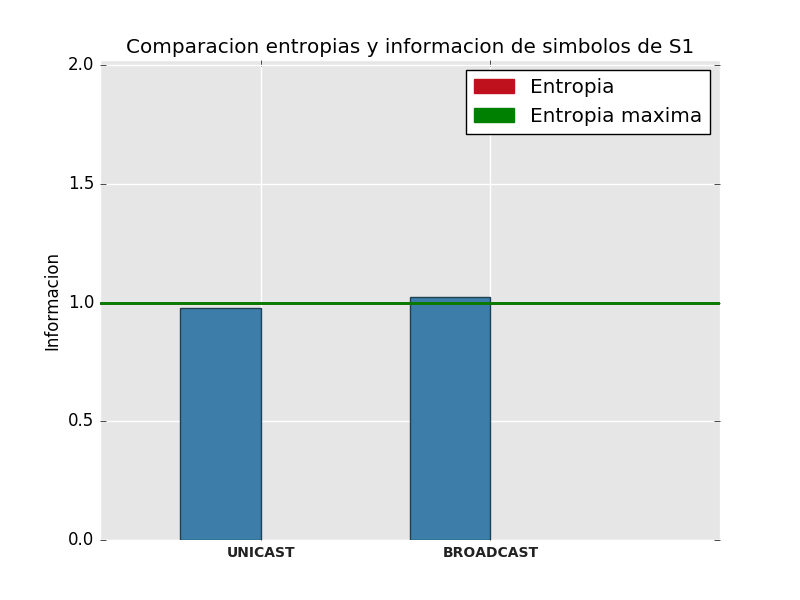
\includegraphics[width=0.45\textwidth]{grafico1-red-taringa.png}
  \caption{Entropia de la fuente}
  \label{}
\end{figure}
Como se puede ver en el gráfico, la entropía llega a ser casi máxima (0,999). 
Esto es debido a que se capturó casi la misma cantida de paquetes UNICAST como de BROADCAST
por lo tanto un símbolo UNICAST proporciona la misma información que un símbolo BROADCAST 

\begin{figure}[h]
  \centering
    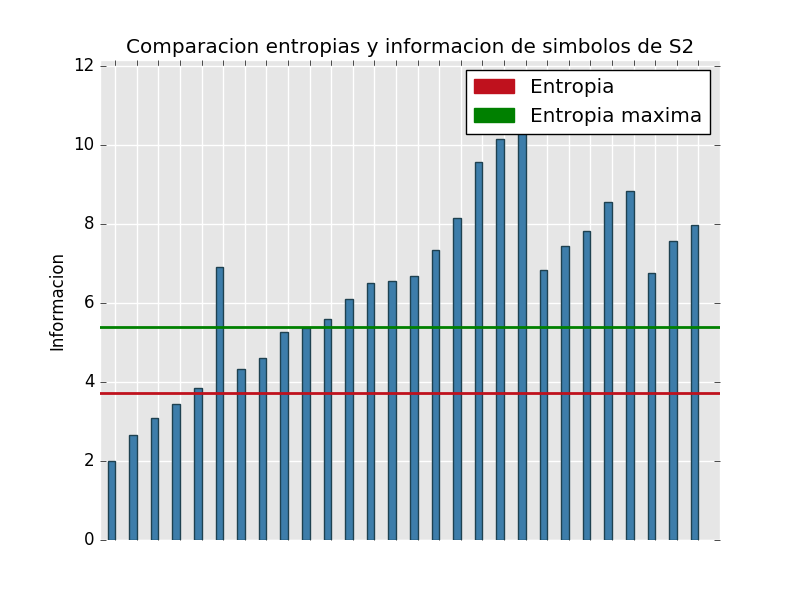
\includegraphics[width=0.45\textwidth]{grafico2-red-taringa.png}
  \caption{Entropia de la fuente}
  \label{}
\end{figure}

    \begin{table}[ht]\begin{center}
      \begin{tabular}{|c|c|}
      \hline
      \textbf{Nodo} & \textbf{Informacion} \\ \hline
      \texttt{192.168.1.224 }& 1.987991 \\ \hline
      \texttt{192.168.1.211 }& 2.666566 \\ \hline
      \texttt{192.168.1.1}& 3.089686 \\ \hline
      \texttt{192.168.1.243}& 3.436136 \\ \hline
      \end{tabular}
      \caption{Nodos destacados}
      \label{Nodos-destacados}
    \end{center}\end{table}

Lo mas probable es que el nodo 192.168.1.1 sea el Default Gateway por la cantidad de información que posee
y además por intuición en su dirección ip, 
Es probable que los demás nodos sean servidores que servicios utilizados por procesos en algún otro host.

\begin{figure}[h]
  \centering
    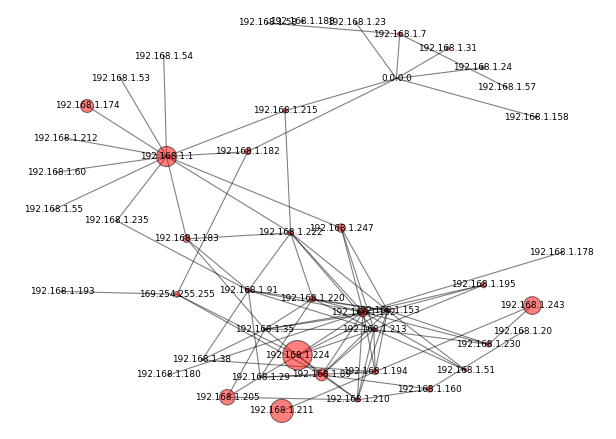
\includegraphics[width=0.45\textwidth]{grafico3-red-taringa.png}
  \caption{Grafo de la red}
  \label{}
\end{figure}

\section{Red Despegar}

Para este experimento se tomo una captura de 20 minutos de la red por cable de despegar.com.

\begin{figure}[h]
  \centering
    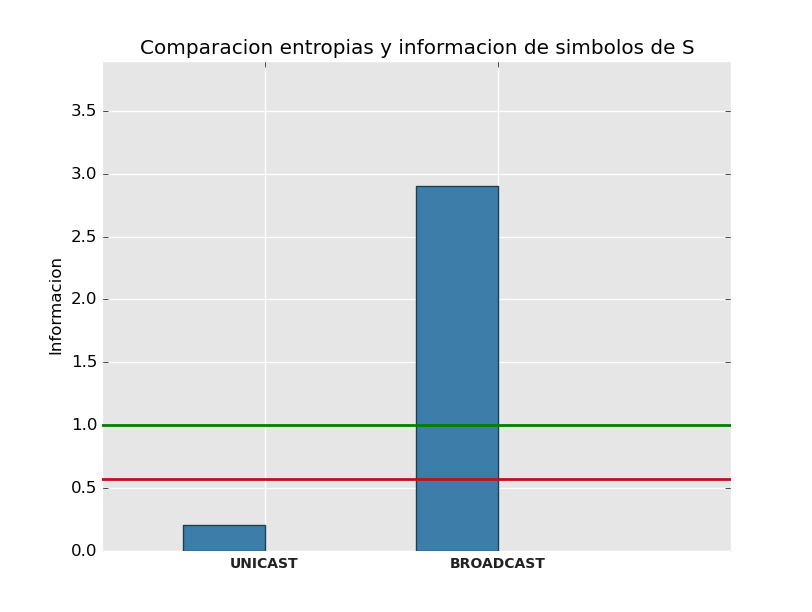
\includegraphics[width=0.45\textwidth]{entropia_red_despegar_s.png}
  \caption{Entropia de la fuente}
  \label{entropia-s}
\end{figure}

Como podemos ver en el gráfico comparativo la entropía no llega a ser máxima. De hecho puede verse en el símbolo $BROADCAST$ proporciona mucha mas información que el símbolo $UNICAST$. 

Por lo que hay un mayor flujo de paquetes Ethernet $UNICAST$ que $BROADCAST$, esto podría deberse a cambios en la topología de la red.


    \begin{table}[ht]\begin{center}
      \begin{tabular}{|c|c|}
      \hline
      \textbf{Nodo} & \textbf{Información} \\ \hline
      \texttt{UNICAST}& 0.207536 \\ \hline
      \texttt{BROADCAST}& 2.899857 \\ \hline
      \end{tabular}
      \caption{Información de los símbolos de S}
      \label{info-simbolos}
    \end{center}\end{table}

La entropia de la fuente da $0.568266518529$ mucho  menor que la maxima entropia que es $1$

El overhead impuesto por la red influencia la entropía de esta fuente.
Por ejemplo, si hubiese mas mensajes $ARP$ $BROADCAST$ la información del símbolo $S_{BROADCAST}$ bajaría haciendo consecuentemente que la entropía de la fuente $S$ se vea modificada.

\begin{figure}[h]
  \centering
    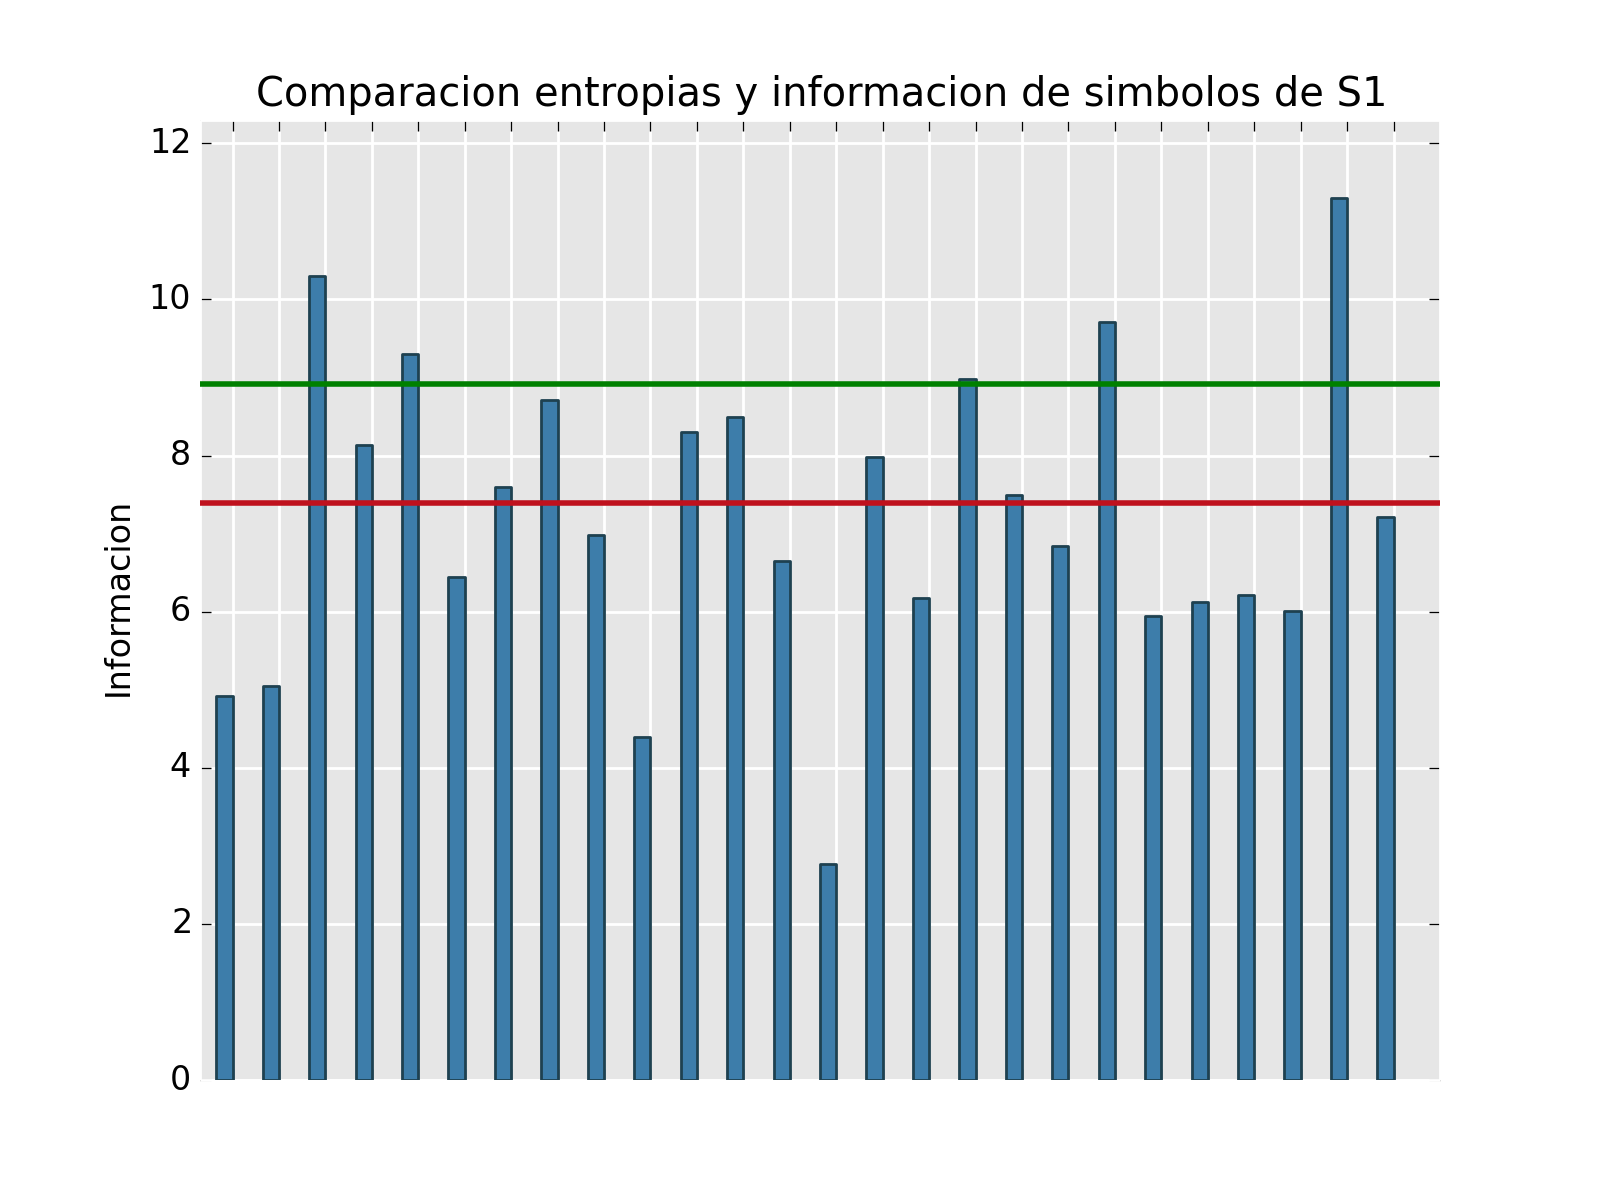
\includegraphics[width=0.45\textwidth]{entropia_red_despegar.png}
  \caption{Entropia de la fuente}
  \label{entropia-s1}
\end{figure}
En este gráfico agrupamos la información puesto que había demasiados símbolos.

En comparación con el resto de los mensajes el tráfico $ARP$ es bajo, el total de paquetes ethernet es $77755$, mientras que los paquetes $ARP$ son $2520$ sólo el 3\%, lo cual indica aparentemente que las tablas que mantienen la información de $ARP$ estan con informacion correcta. 
\\En base al criterio propuesto, se pueden distinguir 16 nodos, que en el grafico se corresponden con las 16 barras que están por debajo de la entroppía de la fuente:   

    \begin{table}[ht]\begin{center}
      \begin{tabular}{|c|c|}
      \hline
      \textbf{Nodo} & \textbf{Informacion} \\ \hline
      \texttt{10.254.213.254}&2.771731\\ \hline
      \texttt{10.254.213.74}&4.392317\\ \hline
      \texttt{10.254.213.103}&4.924169\\ \hline
      \texttt{10.254.95.254}&5.051281 \\ \hline
      \texttt{10.254.213.95}&5.941656 \\ \hline
      \texttt{10.254.213.63}&6.013806 \\ \hline
      \texttt{10.254.213.6}&6.129283 \\ \hline
      \texttt{10.254.213.37}&6.169925 \\ \hline
      \texttt{10.254.213.18}&6.169925 \\ \hline
      \texttt{10.254.213.13}&6.211745 \\ \hline
      \end{tabular}
      \caption{Nodos destacados}
      \label{Nodos-destacados}
    \end{center}\end{table}

Como en nuestra fuente estamos tomando las IPs destino de los paquetes $ARP$ $Who-has$. Esto indíca que estas IPs son muy frecuentes con lo cual se podría pensar en el escenario en que la mayoría de los nodos quiere conocer la MAC del Default Gateway por lo tanto envían tramas $Who-has$ con la dirección destino del mismo. En mi caso particular mi gateway es $10.254.213.254$.


\begin{figure}[h]
  \centering
    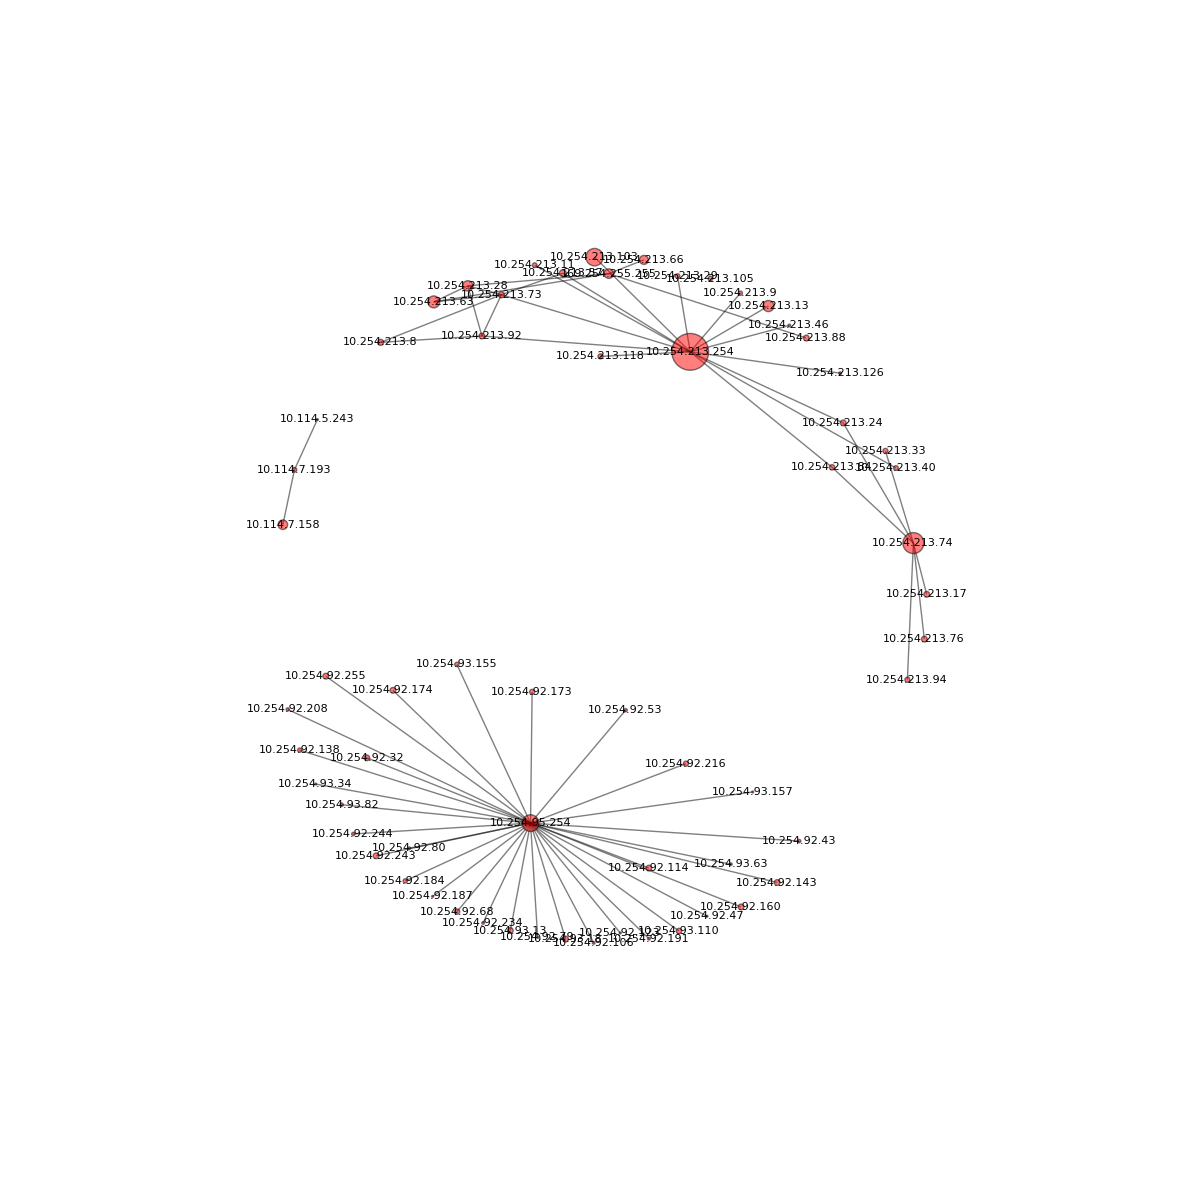
\includegraphics[width=0.45\textwidth]{grafo_red_despegar.png}
  \caption{Grafo de la fuente S1}
  \label{grafo-s1}
\end{figure}
\section{Red de Oficina}

Para este experimento se tomo una captura de 20 minutos de la red Wi-Fi de una oficina, sin conocimientos
previos de esta.

\subsection{Fuente binaria S}

\begin{figure}[H]
  \centering
    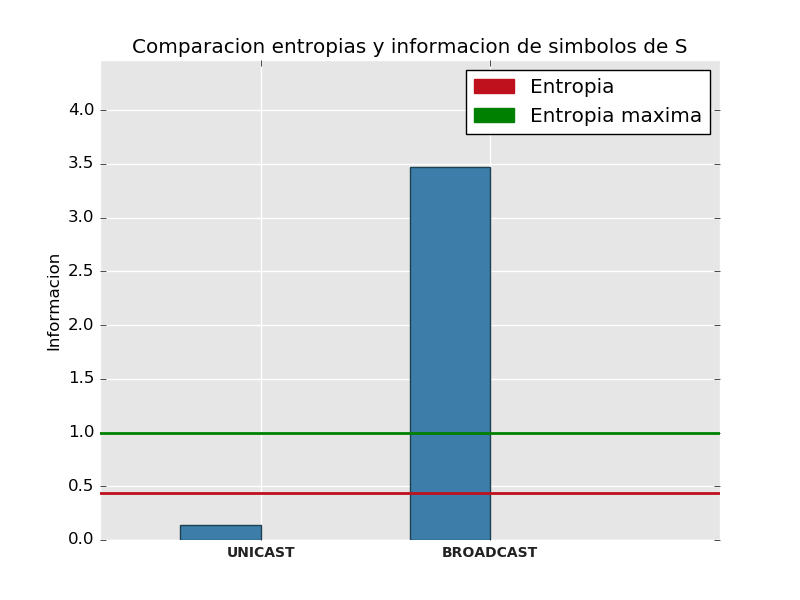
\includegraphics[width=0.45\textwidth]{agutter/gr1.png}
  \caption{Entropia de la fuente S}
  \label{entropia-s-agutter}
\end{figure}

Como podemos ver en el gráfico, y al igual que en casos anteriores, la entropía dista de ser máxima.
De hecho, es claro que el símbolo $BROADCAST$ proporciona considerablemente m\'as información que el
$UNICAST$. 

Podemos entonces deducir que la red cuenta con un mayor flujo de paquetes Ethernet $UNICAST$ que
$BROADCAST$, lo que podría atribuirse a regulares cambios en la topología de la red.

Esto se corresponde a el comportamiento esperado, dado que se trata de una red Wi-fi abierta a la que
probablemente distintos dispositivos se conecten y desconecten con frecuencia, afectando as\'i, la
topolog\'ia de la misma.

\begin{table}[H]\begin{center} %ht
  \begin{tabular}{|c|c|}
    \hline
    \textbf{Nodo} & \textbf{Información} \\ \hline
    \texttt{UNICAST}& 0.136783 \\ \hline
    \texttt{BROADCAST}& 3.466655 \\ \hline
  \end{tabular}
  \caption{Información de los símbolos de S}
  \label{info-simbolos-agutter}
\end{center}\end{table}

Podemos imaginar que el overhead impuesto por la red influencia la entropía de esta fuente, ya que
en caso de tener un menor overhead, la informaci'on del s\'imbolo $S_{BROADCAST}$ se reducir\'ia y
la entrop\'ia de la fuente $S$ aumentar\'ia, acerc\'andola al m\'aximo.

\subsection{Red de Mensajes ARP subyacente}

\begin{figure}[H]
  \centering
    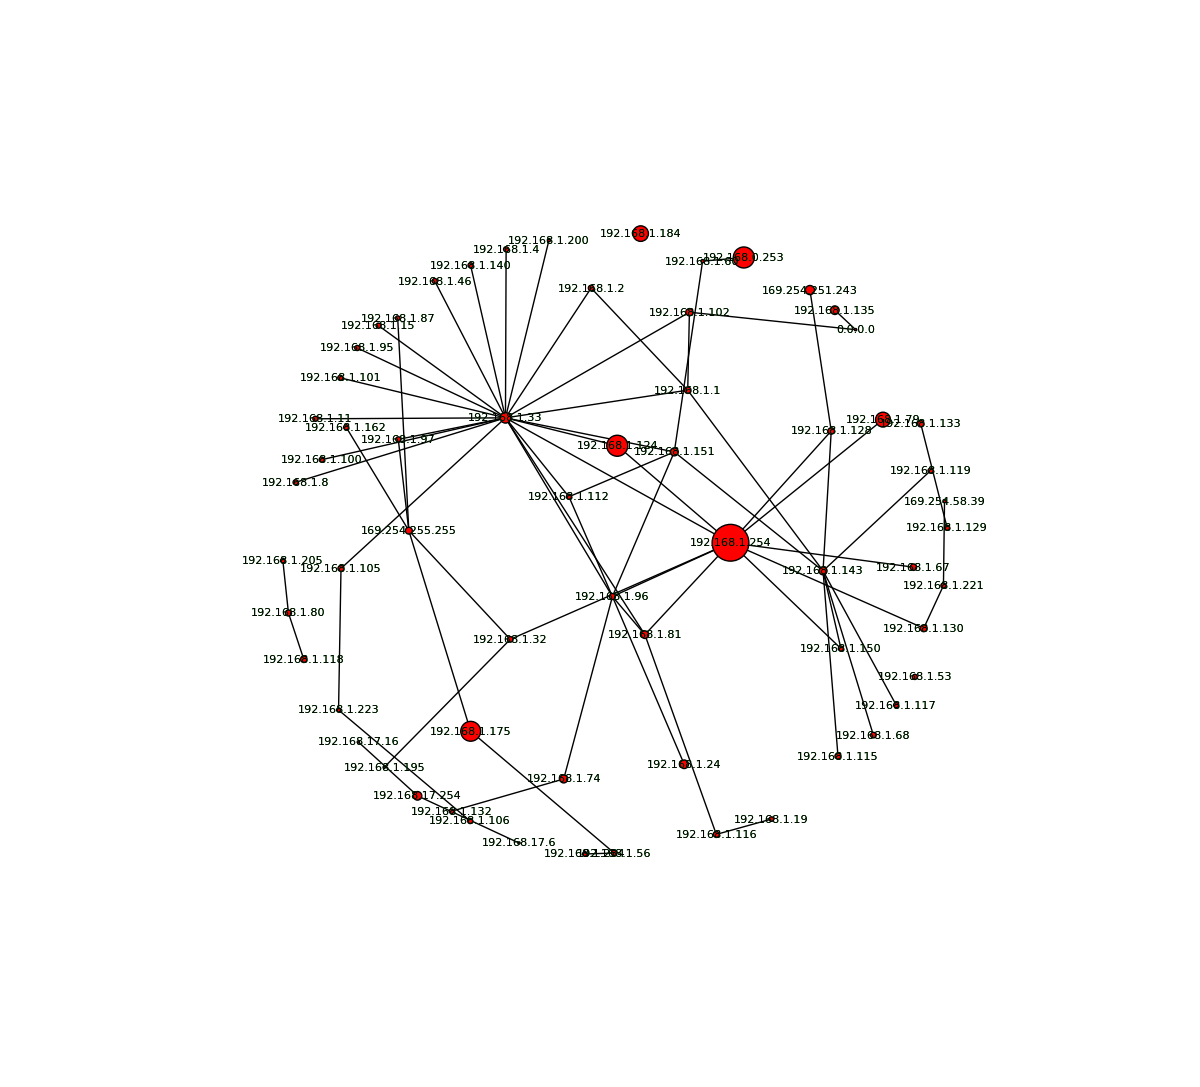
\includegraphics[width=0.45\textwidth]{agutter/gr3.png}
  \caption{Red de Mensajes ARP subyacente}
  \label{grafo-s1-agutter}
\end{figure}

Analizando la cantidad de apariciones (tama\~no) de cada nodo en las tramas ARP y la distribuci\'on de
los v\'ertices, podemos ver que se trata de una red con alto tr\'afico pero mal distribuido:
la gran mayor\'ia de los nodos tiene poca comunicaci\'on. Sin embargo, podemos f\'acilmente distinguir
a 192.168.1.254 como un nodo importante, seguido de 192.168.1.33, 192.168.1.124, 192.168.1.253 y
192.168.1.175.

Dado el tama\~no del nodo 192.168.1.254 y la cantidad de v\'ertices que alcanzan al nodo 192.168.1.33,
podr\'iamos intuir que se trata de posibles gateways de la red, ya que ejercen como centros de gravedad
del grafo, y se comunican con un gran n\'umero de nodos.

Adem\'as, podr\'iamos pensar que el nodo 192.168.1.124 corresponde a la salida de la red ya que tiene
un alto grado de impacto pero solo se comunica con los dos nodos anteriores.


\subsection{Fuente S1}

A continuaci\'on presentamos un gr\'afico comparando la cantidad de informaci\'on de cada s\'imbolo
con la entrop\'ia de la fuente, y una tabla presentando los nodos distinguidos detectados por la
herramienta.

\begin{figure}[H]
  \centering
    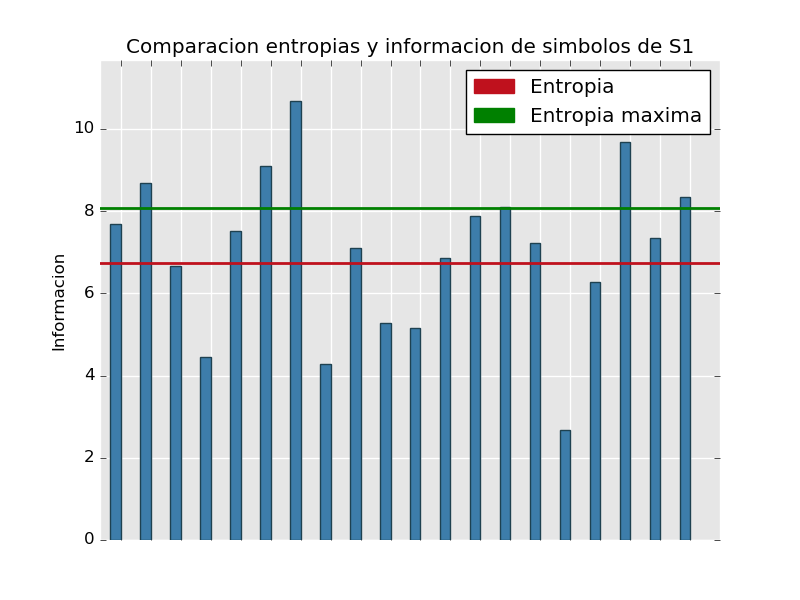
\includegraphics[width=0.45\textwidth]{agutter/gr2.png}
  \caption{Entropia de la fuente S1}
  \label{entropia-s1-agutter}
\end{figure}

\begin{table}[H]\begin{center} %H
  \begin{tabular}{|c|c|}
    \hline
    \textbf{Nodo} & \textbf{Informacion} \\ \hline
    \texttt{192.168.1.254}& 2.672976 \\ \hline
    \texttt{192.168.1.253}& 4.286283 \\ \hline
    \texttt{192.168.1.124}& 4.286283 \\ \hline
    \texttt{192.168.1.175}& 4.449781 \\ \hline
    \texttt{192.168.1.184}& 5.155038 \\ \hline
    \texttt{192.168.1.79}& 5.286283 \\ \hline
    \texttt{192.168.1.33}& 6.286283 \\ \hline
    \texttt{192.254.251.243}& 6.678600 \\ \hline
  \end{tabular}
  \caption{Nodos distinguidos detectados por la herramienta}
  \label{Nodos-distinguidos-agutter}
\end{center}\end{table}

R\'apidamente podemos destacar que los nodos que distinguimos en el punto anterior son tambi\'en detectados
por la herramienta. Esto nos lleva a pensar que detectamos correctamente los posibles gateways de la red.

Observando el gr\'afico, podemos adem\'as ver que son pocos los s\'imbolos con informaci\'on menor a la
entrop\'ia de la fuente, y parecieran corresponderse a los detectados.

Podr\'iamos entonces concluir que el criterio de distinci\'on propuesto es bastante preciso, y quiz\'as
un an\'alisis m\'as fino permitir\'ia encontrar un\'ivocamente los gateways de la red.

%\section{Resultados}
\subsection{Servidor unak.is}
\begin{figure}[H]
  \centering
    \includegraphics[width=0.45\textwidth]{histogramas_rtt/unak-is.png}
  \caption{RTT entre saltos}
  \label{entropia-s}
\end{figure}

\begin{figure}[H]
  \centering
    \includegraphics[width=0.45\textwidth]{histogramas_thompson/unak-is.png}
  \caption{RTT }
  \label{entropia-s}
\end{figure}

\begin{figure}[H]
  \centering
    \includegraphics[width=0.45\textwidth]{grafico-rutas/unak-is.png}
  \caption{Gráfico de la ruta}
  \label{entropia-s}
\end{figure}




\subsection{Servidor unak.is}
\begin{figure}[H]
  \centering
    \includegraphics[width=0.45\textwidth]{histogramas_rtt/unak-is.png}
  \caption{RTT entre saltos}
  \label{entropia-s}
\end{figure}

\begin{figure}[H]
  \centering
    \includegraphics[width=0.45\textwidth]{histogramas_thompson/unak-is.png}
  \caption{RTT }
  \label{entropia-s}
\end{figure}

\begin{figure}[H]
  \centering
    \includegraphics[width=0.45\textwidth]{grafico-rutas/unak-is.png}
  \caption{Gráfico de la ruta}
  \label{entropia-s}
\end{figure}




\subsection{Servidor unis.no}
\begin{figure}[H]
  \centering
    \includegraphics[width=0.45\textwidth]{histogramas_rtt/unis-no.png}
  \caption{RTT entre saltos}
  \label{entropia-s}
\end{figure}

\begin{figure}[H]
  \centering
    \includegraphics[width=0.45\textwidth]{histogramas_thompson/unis-no.png}
  \caption{RTTs Normailzados comparados con el valor Thompson}
  \label{entropia-s}
\end{figure}

\begin{figure}[H]
  \centering
    \includegraphics[width=0.45\textwidth]{grafico-rutas/unis-no.png}
  \caption{Gráfico de la ruta}
  \label{entropia-s}
\end{figure}




\subsection{Servidor www.fu-berlin.de}
\begin{figure}[H]
  \centering
    \includegraphics[width=0.45\textwidth]{histogramas_rtt/www-fu-berlin-de.png}
  \caption{RTT entre saltos}
  \label{entropia-s}
\end{figure}

\begin{figure}[H]
  \centering
    \includegraphics[width=0.45\textwidth]{histogramas_thompson/www-fu-berlin-de.png}
  \caption{RTTs Normailzados comparados con el valor Thompson}
  \label{entropia-s}
\end{figure}

\begin{figure}[H]
  \centering
    \includegraphics[width=0.45\textwidth]{grafico-rutas/www-fu-berlin-de.png}
  \caption{Gráfico de la ruta}
  \label{entropia-s}
\end{figure}




\subsection{Servidor www.kstu.kz}
\begin{figure}[H]
  \centering
    \includegraphics[width=0.45\textwidth]{histogramas_rtt/www-kstu-kz.png}
  \caption{RTT entre saltos}
  \label{entropia-s}
\end{figure}

\begin{figure}[H]
  \centering
    \includegraphics[width=0.45\textwidth]{histogramas_thompson/www-kstu-kz.png}
  \caption{RTTs Normailzados comparados con el valor Thompson}
  \label{entropia-s}
\end{figure}

\begin{figure}[H]
  \centering
    \includegraphics[width=0.45\textwidth]{grafico-rutas/www-kstu-kz.png}
  \caption{Gráfico de la ruta}
  \label{entropia-s}
\end{figure}




\subsection{Servidor www.uq.edu.au}
\begin{figure}[H]
  \centering
    \includegraphics[width=0.45\textwidth]{histogramas_rtt/www-uq-edu-au.png}
  \caption{RTT entre saltos}
  \label{entropia-s}
\end{figure}

\begin{figure}[H]
  \centering
    \includegraphics[width=0.45\textwidth]{histogramas_thompson/www-uq-edu-au.png}
  \caption{RTTs Normailzados comparados con el valor Thompson}
  \label{entropia-s}
\end{figure}

\begin{figure}[H]
  \centering
    \includegraphics[width=0.45\textwidth]{grafico-rutas/www-uq-edu-au.png}
  \caption{Gráfico de la ruta}
  \label{entropia-s}
\end{figure}




\subsection{Servidor keu.kz}
\begin{figure}[H]
  \centering
    \includegraphics[width=0.45\textwidth]{histogramas_rtt/keu-kz.png}
  \caption{RTT entre saltos}
  \label{entropia-s}
\end{figure}

\begin{figure}[H]
  \centering
    \includegraphics[width=0.45\textwidth]{histogramas_thompson/keu-kz.png}
  \caption{RTTs Normailzados comparados con el valor Thompson}
  \label{entropia-s}
\end{figure}

\begin{figure}[H]
  \centering
    \includegraphics[width=0.45\textwidth]{grafico-rutas/keu-kz.png}
  \caption{Gráfico de la ruta}
  \label{entropia-s}
\end{figure}




\subsection{Servidor kgiu.kz}
\begin{figure}[H]
  \centering
    \includegraphics[width=0.45\textwidth]{histogramas_rtt/kgiu-kz.png}
  \caption{RTT entre saltos}
  \label{entropia-s}
\end{figure}

\begin{figure}[H]
  \centering
    \includegraphics[width=0.45\textwidth]{histogramas_thompson/kgiu-kz.png}
  \caption{RTTs Normailzados comparados con el valor Thompson}
  \label{entropia-s}
\end{figure}

\begin{figure}[H]
  \centering
    \includegraphics[width=0.45\textwidth]{grafico-rutas/kgiu-kz.png}
  \caption{Gráfico de la ruta}
  \label{entropia-s}
\end{figure}




\subsection{Servidor site.u.pereslavl.ru}
\begin{figure}[H]
  \centering
    \includegraphics[width=0.45\textwidth]{histogramas_rtt/site-u-pereslavl-ru.png}
  \caption{RTT entre saltos}
  \label{entropia-s}
\end{figure}

\begin{figure}[H]
  \centering
    \includegraphics[width=0.45\textwidth]{histogramas_thompson/site-u-pereslavl-ru.png}
  \caption{RTTs Normailzados comparados con el valor Thompson}
  \label{entropia-s}
\end{figure}

\begin{figure}[H]
  \centering
    \includegraphics[width=0.45\textwidth]{grafico-rutas/site-u-pereslavl-ru.png}
  \caption{Gráfico de la ruta}
  \label{entropia-s}
\end{figure}




\subsection{Servidor udsu.ru}
\begin{figure}[H]
  \centering
    \includegraphics[width=0.45\textwidth]{histogramas_rtt/udsu-ru.png}
  \caption{RTT entre saltos}
  \label{entropia-s}
\end{figure}

\begin{figure}[H]
  \centering
    \includegraphics[width=0.45\textwidth]{histogramas_thompson/udsu-ru.png}
  \caption{RTTs Normailzados comparados con el valor Thompson}
  \label{entropia-s}
\end{figure}

\begin{figure}[H]
  \centering
    \includegraphics[width=0.45\textwidth]{grafico-rutas/udsu-ru.png}
  \caption{Gráfico de la ruta}
  \label{entropia-s}
\end{figure}




\subsection{Servidor www.uae.ma}
\begin{figure}[H]
  \centering
    \includegraphics[width=0.45\textwidth]{histogramas_rtt/www-uae-ma.png}
  \caption{RTT entre saltos}
  \label{entropia-s}
\end{figure}

\begin{figure}[H]
  \centering
    \includegraphics[width=0.45\textwidth]{histogramas_thompson/www-uae-ma.png}
  \caption{RTTs Normailzados comparados con el valor Thompson}
  \label{entropia-s}
\end{figure}

\begin{figure}[H]
  \centering
    \includegraphics[width=0.45\textwidth]{grafico-rutas/www-uae-ma.png}
  \caption{Gráfico de la ruta}
  \label{entropia-s}
\end{figure}




\subsection{Servidor bifrost.is}
\begin{figure}[H]
  \centering
    \includegraphics[width=0.45\textwidth]{histogramas_rtt/bifrost-is.png}
  \caption{RTT entre saltos}
  \label{entropia-s}
\end{figure}

\begin{figure}[H]
  \centering
    \includegraphics[width=0.45\textwidth]{histogramas_thompson/bifrost-is.png}
  \caption{RTTs Normailzados comparados con el valor Thompson}
  \label{entropia-s}
\end{figure}

\begin{figure}[H]
  \centering
    \includegraphics[width=0.45\textwidth]{grafico-rutas/bifrost-is.png}
  \caption{Gráfico de la ruta}
  \label{entropia-s}
\end{figure}




\subsection{Servidor birmingham.ac.uk}
\begin{figure}[H]
  \centering
    \includegraphics[width=0.45\textwidth]{histogramas_rtt/birmingham-ac-uk.png}
  \caption{RTT entre saltos}
  \label{entropia-s}
\end{figure}

\begin{figure}[H]
  \centering
    \includegraphics[width=0.45\textwidth]{histogramas_thompson/birmingham-ac-uk.png}
  \caption{RTTs Normailzados comparados con el valor Thompson}
  \label{entropia-s}
\end{figure}

\begin{figure}[H]
  \centering
    \includegraphics[width=0.45\textwidth]{grafico-rutas/birmingham-ac-uk.png}
  \caption{Gráfico de la ruta}
  \label{entropia-s}
\end{figure}
%\section{Conclusiones}

Escuchar y analizar el tráfico ARP de una red a la cual uno esta conectado, 
es una forma efectiva de conocer la topología de la misma hasta el primer salto del router.
Mediante el cálculo de la entropía de la red y la información de las direcciónes de los hosts, se puede obtener dicho resultado.\\
En los casos estudiados, pudimos observar que los simbolos con información menor a la entropía se corresponden con el conjunto de simbolos distinguidos, entre los cuales se encuentran los gateways de la red, pero este metodo no es preciso en el sentido que da otros nodos que no son gateways.\\
Pensamos que si tendriamos mas redes con informacion precisa de los gateways, podriamos encontrar un rango de entropia que ajuste mejor para detectar los gateways, pero no contamos con tal información.\\
Tambien vimos que para redes chicas pasa que el nodo distinguido puede no dar el gateway. Esto paso analizando las redes de nuestras casas. Tambien coincide que la fuente s1 tiene entropia casi maxima, lo cual indica que hay mucho desorden. Ahora a medida que la redes crecen en tamaño vemos que a entropia baja y se distinguen mejor los gateways. 

%\input{anexos.tex}

% do the biliography:

\bibliographystyle{IEEEbib}
\bibliography{my-bibliography-file}

\begin{thebibliography}{1}

\bibitem{wireshark}
http://www.wireshark.org/
\bibitem{scapy}
http://en.wikipedia.org/wiki/Scapy
\bibitem{python}
https://www.python.org/
\bibitem{ieee}
https://www.ieee.org
\end{thebibliography}


% where ``my-bibliography-file.bib'' is the name of the file with all the 
% BibTeX entries.

% do the biographies...
% If you want a picture with your biography, then specify the name of
% the postscript file in square brackets. That is, uncomment the
% following three lines and change the name of "face.ps" to the name of 
% your file.
%\begin{biography}[face.ps]{Gregory L. Plett}
%  A bio with a face...
%\end{biography}

%----------------------------------------------------------------------
% FIGURES
%----------------------------------------------------------------------
% There are many ways to include figures in the text. We will assume
% that the figure is some sort of EPS file.
%
% The outdated packages epsfig and psfig allow you to insert figures
% like: \psfig{filename.eps} These should really be done now using the
% \includegraphics{filename.eps} command.  
%
% i.e.,
%
% \includegraphics{file.eps}
%
% whenever you want to include the EPS file 'file.eps'. There are many
% options for the includegraphics command, and are outlined in the
% on-line documentation for the "graphics bundle". Using the options,
% you can specify the height, total height (height+depth), width, scale,
% angle, origin, bounding box "bb",view port, and can trim from around
% the sides of the figure. You can also force LaTeX to clip the EPS file
% to the bounding box in the file. I find that I often use the scale,
% trim and clip commands.
% 
% \includegraphics[scale=0.6,trim=0 0 0 0,clip=]{file.eps}
% 
% which magnifies the graphics by 0.6 (If I create a graphics for an
% overhead projector transparency, I find that a magnification of 0.6
% makes it look much better in a paper), trims 0 points off
% of the left, bottom, right and top, and clips the graphics. If the
% trim numbers are negative, space is added around the figure. This can
% be useful to help center the graphics, if the EPS file bounding box is
% not quite right.
% 
% To center the graphics,
% 
% \begin{center}
% \includegraphics...
% \end{center}
% 
% I have not yet written good documentation for this, but another 
% package which helps in figure management is the package ieeefig.sty,
% available at: http://www-isl.stanford.edu/people/glp/ieee.shtml
% Specify:
% 
%\usepackage{ieeefig} 
% 
% in the preamble, and whenever you want a figure,
% 
%\figdef{filename}
% 
% where, filename.tex is a LaTeX file which defines what the figure is.
% It may be as simple as
% 
% \inserteps{filename.eps}
%
% or
% \inserteps[includegraphics options]{filename.eps}
% 
% or may be a very complicated LaTeX file. 

\end{document}
